\documentclass[12pt]{article}
\usepackage{pictex,amsmath,amsfonts,fullpage,amssymb,amsthm}
\usepackage{graphics,graphicx}
\usepackage{fancyhdr}
\usepackage{multirow}
\usepackage{algorithm,algorithmic}
\usepackage{listingsutf8}
\usepackage{lmodern}

\setlength{\voffset}{-0.25in}
\setlength{\headsep}{+0.5in}
\setlength{\parskip}{1em}
\setlength{\parindent}{0em}

\def\vu{\mathbf{u}}
\def\vv{\mathbf{v}}
\def\vs{\mathbf{s}}
\def\vb{\mathbf{b}}
\def\vw{\mathbf{w}}

\renewcommand{\implies}{\rightarrow}
\renewcommand{\lor}{\vee}
\renewcommand{\land}{wedge}
\renewcommand{\iff}{\leffrightarrow}
\newcommand{\TRUE}{\mathbf{T}}
\newcommand{\FALSE}{\mathbf{F}}
\newcommand{\universe}{\mathcal{U}}

\usepackage{xcolor}
\usepackage{mdframed}
\usepackage[utf8]{vietnam}
\usepackage[utf8]{inputenc}
\usepackage{textcomp}
\usepackage[T1]{fontenc}

\newmdenv[linecolor=red,skipabove=\topsep,skipbellow=\topsep,leftmargin=5pt,rightmargin=-5pt,innerleftmargin=5pt,innerrightmargin=5pt]{mybox}

\begin{document}
\begin{center}
\textbf{Some Python code}
\end{center}
\section{Subsetting List}
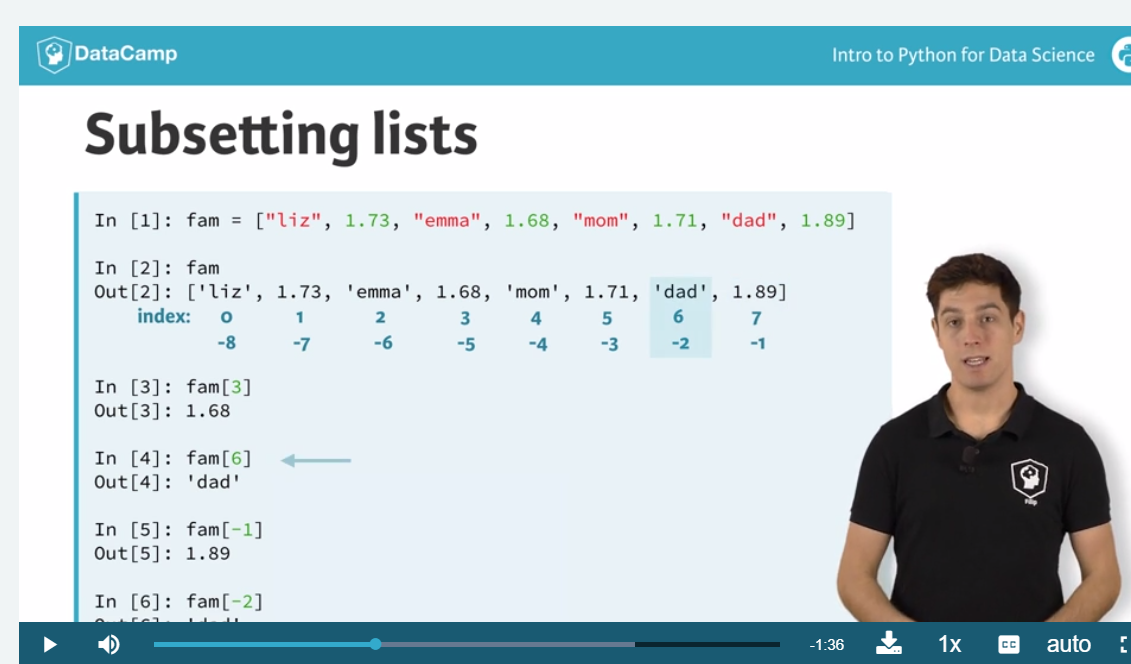
\includegraphics[scale=0.8]{hinh}
\textbf{List Slicing :}
\begin{lstlisting}
list[`liz', 1.73, `emma', 1.68, `mom', 1.71, `dad', 1.89]
list[3:5]
//Terminate:
[1.68, `mom'
\end{lstlisting}
\section{Add to list}
\begin{lstlisting}
# Create the areas list and make some changes
areas = ["hallway", 11.25, "kitchen", 18.0, "chill zone", 20.0,
         "bedroom", 10.75, "bathroom", 10.50]

# Add poolhouse data to areas, new list is areas_1
areas_1 = areas + ["poolhouse", 24.5]
print(areas_1) 

# Add garage data to areas_1, new list is areas_2
areas_2 = areas_1 + ["garage", 15.45]
print(areas_2)
\end{lstlisting}
\section{Delete list element}
\begin{lstlisting}
x = ["a", "b", "c", "d"]
del(x[1])
print(x)
\end{lstlisting}
Then we have:[`b',`c',`d']
\section{Inner workings on lists}
\begin{lstlisting}
# Create list areas
areas = [11.25, 18.0, 20.0, 10.75, 9.50]

# Create areas_copy
areas_copy = areas

# Change areas_copy
areas_copy[0] = 5.0

# Print areas
print(areas)
\end{lstlisting}
\section{Print type of Function}
\begin{lstlisting}
result = type(3.0)
# Assign type of function 3.0 for variable `result'
print(result)
# Print `result'
\end{lstlisting}
\pagebreak
\section{Length of type}
\begin{lstlisting}[frame=single]
result = 3.0 + 2.5
# Assign the value for result
print(len(result))
# Print the length of `result'
\end{lstlisting}
\section{Show Help in Python}
\begin{lstlisting}
# Show sth about the code you need
help(function,...)
\end{lstlisting}
\section{Sorted}
\begin{lstlisting}
# sorted() take three arguements(iterable,key,reverse)
# If you don't spectify anything in sorted() then key=None, reverse=true
(decending order)
sorted(iterable, [ key], [reverse=])
\end{lstlisting}
\section{Upper Method}
\begin{lstlisting}
 # Upper String [str.upper]
room = `poolhouses'
room_up = room.upper()
 # Print room_up
print(room_up)
\end{lstlisting}
\section{Count Method}
\begin{lstlisting}
 # Count the string str.count([substr or str], start=, end=len(str))
 print(room.count(``o''))
\end{lstlisting}
\section{List Method}
\begin{lstlisting}
 # Index Method
areas = [11.25, 18.0, 20.0, 10.75, 9.50]
 # Print Index of 20.0
print(areas.index(12.0))
 # Print Count of 14.5
print(areas.count(14.5))
 # Add an elemenet to the list it is called on
print(areas.append(23.00))
 # Remov ean element to the list that matches the input
print(areas.remove(10.75))
 #Reverse the order of the elements in the list it is called on.
print(areas.reverse())
\end{lstlisting}
\section{Numpy}
\begin{lstlisting}
# Create list baseball
baseball = [180, 215, 210, 210, 188, 176, 209, 200]

# Import the numpy package as np
import numpy as np

# Create a numpy array from baseball: np_baseball
np_baseball = np.array(baseball)

# Print out type of np_baseball
print(type(np_baseball))
# Print out dtype of np_baseball
print(type(np_baseball.dtype))
\end{lstlisting}
\pagebreak
\begin{center}
\textbf{NumPy in Python}
\end{center}
\section{Numpy Array}
\begin{lstlisting}
# To use NumPy array we import NumPy package
import numpy as np
# create a list
height = [12.45,78.90,34.56,56.78]
# Use np.array(...) to make NumPy array
np_height = np.array(height)
# We can add function in array
np_height_m = np_height * 0.05
print(np_height_m)
\end{lstlisting}
\end{document}